\documentclass[12pt]{article}

\newcommand{\myname}{Tan Yee Jian (A0190190L)}
\newcommand{\mytitle}{FSC2101 Final Term Paper\\(Question A)}
\title{\mytitle}
\author{\myname}
\date{\today}

\usepackage[a4paper, total={6in, 9.7in}]{geometry}
\usepackage[utf8]{inputenc}
\usepackage[T1]{fontenc}
\usepackage{textcomp}
\usepackage{amsmath, amssymb, amsthm}
\theoremstyle{plain}
% \usepackage[outputdir=tmp]{minted}
% \usepackage{lmodern}
\usepackage{tgpagella}
\usepackage{fancyhdr}
\usepackage{lastpage}
\usepackage{chemformula}
\usepackage{graphicx}
\usepackage{subfigure}
\pagestyle{fancy}
\fancyhf{}
% \rhead{Page \thepage/\pageref{LastPage}}
\rhead{Page \thepage}
\lhead{\myname}
\chead{\mytitle}

\newcommand{\pmat}[1]{ \begin{pmatrix}#1\end{pmatrix} }
\newcommand{\seqn}[1]{(#1)^\infty_{n=1}}
\newcommand{\seqk}[1]{(#1)^\infty_{k=1}}
% (series term): returns a series with counter n=1 to \infty.
\newcommand{\infsrsn}[1]{\sum\limits^\infty_{n=1}#1}
\newcommand{\infsrsk}[1]{\sum\limits^\infty_{k=1}#1}
\newcommand{\R}{\mathbb{R}}
\newcommand{\N}{\mathbb{N}}
\newcommand{\Q}{\mathbb{Q}}
\newcommand{\Z}{\mathbb{Z}}
\newcommand{\C}{\mathbb{C}}
\newcommand{\F}{\mathbb{F}}
\newcommand{\cmm}{C(M_1,M_2)}
\newcommand{\met}[1]{\langle M_{#1},\rho_{#1}\rangle}
\newcommand{\ntoinf}{\limits_{n\to\infty}}
\newcommand{\ktoinf}{\limits_{k\to\infty}}
% \newcommand{\onetoinf}[]{^\infty_{n=1}}
\newcommand{\limn}[1]{\lim\ntoinf #1}
\newcommand{\limk}[1]{\lim\ktoinf #1}

\DeclareMathOperator{\spn}{span}
\DeclareMathOperator{\diam}{diam}

\begin{document}
\maketitle
% \tableofcontents
\section{Introduction}
To investigate a recent innovation/finding in forensic science (Question A), I
will review a paper from the latest issue (Volume 329) from Forensic Science
International, of the title ``Assessing optical remote sensing for grave
detection''\\
\cite{SILVANCARDENAS2021111064}.


% \subsection{Background}
% \label{subsec:background}
% The ongoing drug war in Mexico has caused a high homicide rate. Nearly 100,000
% people are missing, and these people, sometimes executed rivals or kidnapped
% victims, were disposed and buried in clandestine graves. It is of forensic
% importance to search for and determine the existence of these graves with easy
% and reliable ways.

\subsection{Background}
\label{subsec:background}
Resisitivity meters, magnetometers, thermography cameras and ground penetrating
radars have been used to search for human remains buried 0m to 10m below surface
\cite{SILVANCARDENAS2021111064}. These methods are non-destructive and
relatively fast, but can only cover very small areas due to their intense field
deployment. In Mexico where clandestine graves are prevalent due to the raging
drug war \cite{reuters_2020}, the authors investigated 3 remote sensing methods
that can scan large pieces of land in a short time, namely, multi/hyperspectral
sensors, thermography sensors, and unmanned aerial vehicles (UAV).

\subsection{Methods of Measurements}
\label{subsec:methods}
\begin{enumerate}
  \item \textbf{Multispectral cameras }are cameras that detect up to 12 spectra
        bands of light (compared to only 3 on conventional cameras), and up to
        hundreds of spectra bands on a \textbf{hyperspectral camera}. These
        cameras can capture much more details than typical cameras.
  \item \textbf{Thermography sensors}, or thermal cameras are common in the
        post-Covid world, especially used to measure human temperatures in
        crowded areas.
  \item Finally, \textbf{UAV photogrammetry} aims to capture full images of the
        site using a UAV, which is cheap and effective.
\end{enumerate}

\begin{figure}[h]%
\centering
\subfigure[Multispectral]{%
\label{fig:multi}%
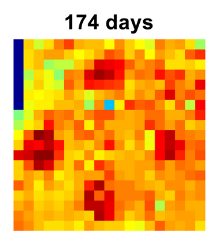
\includegraphics[height=4cm]{multi.png}}%
\quad
\subfigure[UAV]{%
\label{fig:uav}%
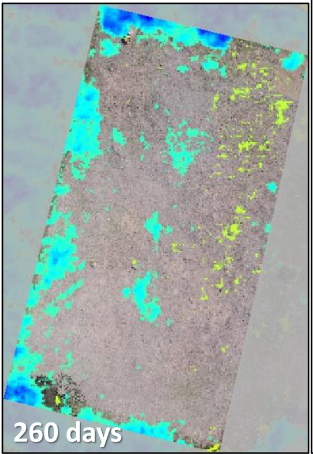
\includegraphics[height=4cm]{uav.png}}%
\quad
\subfigure[Thermograph]{%
\label{fig:thermo}%
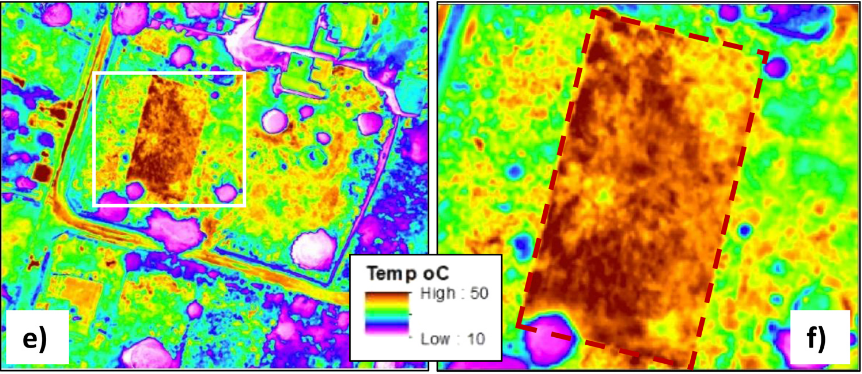
\includegraphics[height=3cm]{thermal.png}}%
\caption{Multispectral, Thermal and UAV images \cite{SILVANCARDENAS2021111064}}
\end{figure}

\section{Questions investigated and their answers}
\label{sec:questions}
The authors carried out 2 controlled experiments of burying pig corpses in 2
sites in Mexico, which answers question \ref{subsec:confounding}, and the other
questions (\ref{subsec:spectral}, \ref{subsec:thermal}, \ref{subsec:uav})
respectively.


\subsection{What happens if there are confounding factors like clothes on the
  corpses, or lime in the land?}
\label{subsec:confounding}
\cite{SILVANCARDENAS2021111064} concluded:
\begin{enumerate}
  \item A larger grave will be at least as spectrally separable than a smaller
        grave.
  \item The presence of lime (\ch{CaO} and/or \ch{Ca(OH)_{2}}) does not reduce the
        spectral separability of the grave.
  \item The presence of clothes does not reduce the spectral separability of the
        grave.
  \item Lowering the resolution of the multispectral cameras can only reduce the
        spectral separability.
\end{enumerate}

\subsection{Can hyperspectral and multispectral sensors detect graves?}
\label{subsec:spectral}
Yes, given enough time for the vegetation to grow. Decaying bodies provide ample
nutrients such as Nitrogen (\ch{N}) which can directly influence chlorophyll
content in plants and make them green. However, decay of bodies depends on the
climate and microbe; in this paper, 3.5 to 4 months were needed (under the
Mexican warm climate) to see significant change in the data. See figure
\ref{fig:multi}.


\subsection{Can thermal imagery detect graves?}
\label{subsec:thermal}
Yes, due the voids created by the graves after the bodies have decomposed
(Figure \ref{fig:thermo}). However, there are anomalies such as plastic which
would affect the experiment result, but the authors noted it as a useful
discovery since it is common for body parts to be wrapped in plastic before
buried or discarded.

\subsection{Can UAV-photogrametry detect graves?}
\label{subsec:uav}
Yes, but only to a certain extent. It can detect terrain changes (such as
depresion in the surface due to soil compression and body decomposition in a
grave, figure \ref{fig:uav}), but because it is unable to penetrate vegetation
(unlike LiDAR), it ``can only record the upper vegetation canopy''. However, due to
its cost-effectiveness, UAVs are ``useful for documenting the state of a search
site'' \cite{SILVANCARDENAS2021111064}.


\bibliographystyle{apalike}
\bibliography{references}
\end{document}
